\def\DoNotLoadEpstopdf{}
\documentclass[tikz,border=4pt]{standalone}
% Shared style for the technical appendix figures (2026-10-26).
% Builds on the proposal's figstyle.tex (same fonts, colors, and box styles) and adds
% one encoding for development status, used the same way in every appendix figure.
%   built and tested   solid border (the proposal's normal box styles)
%   built, no test     solid border, and the box text says "no test"
%   specified          dashed border            -> add the key  spec
%   planned            dotted grey border        -> use the style planned
%   no code (by hand)  dotted arrow              -> add the key  byhand
%   outside the artifact  solid grey border      -> use the style outside
% Shared style for proposal figures (2026-10-22 visuals pass).
% Sized to print at 6.5 in (16.5 cm) wide; body text 9 pt sans, nothing below 8 pt.
\usepackage[T1]{fontenc}
\usepackage[scaled=0.95]{helvet}
\renewcommand{\familydefault}{\sfdefault}
\usepackage{xcolor}
\usetikzlibrary{arrows.meta,positioning,calc,patterns.meta}
\definecolor{cink}{HTML}{16191F}
\definecolor{cmuted}{HTML}{4B5563}
\definecolor{cslate}{HTML}{2F4858}
\definecolor{cslatefill}{HTML}{E9EFF3}
\definecolor{cbrass}{HTML}{7A5C12}
\definecolor{cbrassfill}{HTML}{F5EFDE}
\definecolor{cred}{HTML}{8C2F39}
\definecolor{credfill}{HTML}{F8E9EA}
\definecolor{cgreen}{HTML}{235C53}
\definecolor{cgreenfill}{HTML}{E3F0EC}
\definecolor{caudit}{HTML}{5B3A8E}
\definecolor{cauditfill}{HTML}{EFE9F6}
\definecolor{cghost}{HTML}{6B7280}
\definecolor{cghostfill}{HTML}{F3F4F6}
\tikzset{
  >={Triangle[length=5pt,width=4.5pt]},
  box/.style={draw, rounded corners=1.5pt, line width=0.8pt, align=center, inner sep=4pt, font=\fontsize{9}{11}\selectfont},
  sub/.style={font=\fontsize{8}{9.6}\selectfont, text=cmuted},
  ai/.style={box, draw=cbrass, fill=cbrassfill, text=cbrass},
  ver/.style={box, draw=cred, fill=credfill, text=cred},
  pipe/.style={box, draw=cslate, fill=cslatefill, text=cslate},
  prod/.style={box, draw=cslate, fill=cslate, text=white},
  person/.style={box, draw=cink, fill=white, text=cink},
  ghost/.style={box, draw=cghost, fill=cghostfill, text=cghost, dash pattern=on 3pt off 2pt},
  flow/.style={->, line width=0.8pt},
}

\renewcommand{\ttdefault}{lmtt}% vector typewriter font (same design as the default, not a bitmap)
\tikzset{
  spec/.style={dash pattern=on 3pt off 2pt},
  planned/.style={box, draw=cghost, fill=cghostfill, text=cghost, dash pattern=on 0.9pt off 1.6pt},
  outside/.style={box, draw=cghost, fill=white, text=cghost},
  byhand/.style={dash pattern=on 0.9pt off 1.6pt},
  prog/.style={font=\fontsize{8}{9.6}\selectfont\ttfamily},
  legendbox/.style={draw, rounded corners=1pt, line width=0.8pt, minimum width=0.55cm, minimum height=0.32cm, inner sep=0pt},
  legendtext/.style={font=\fontsize{8}{9.6}\selectfont, text=cink, anchor=west, inner sep=1pt},
}
% \statuslegend{x}{y} draws the four-item status legend with its left edge at (x,y).
\newcommand{\statuslegend}[2]{%
  \begin{scope}[shift={(#1,#2)}]
    \node[legendbox, draw=cink, fill=white] (lg1) at (0.275,0) {};
    \node[legendtext] at (0.65,0) {Built and tested};
    \node[legendbox, draw=cink, fill=white, spec] (lg2) at (3.35,0) {};
    \node[legendtext] at (3.725,0) {Specified};
    \node[legendbox, draw=cghost, fill=cghostfill, dash pattern=on 0.9pt off 1.6pt] (lg3) at (5.75,0) {};
    \node[legendtext] at (6.125,0) {Planned};
    \node[legendbox, draw=cghost, fill=white] (lg4) at (7.85,0) {};
    \node[legendtext] at (8.225,0) {Outside the research artifact};
  \end{scope}}

% Figure A2 of the 10/26c appendix: the reproducible pipeline as a build-only layer. Design only, no status.
\begin{document}
\hyphenpenalty=10000
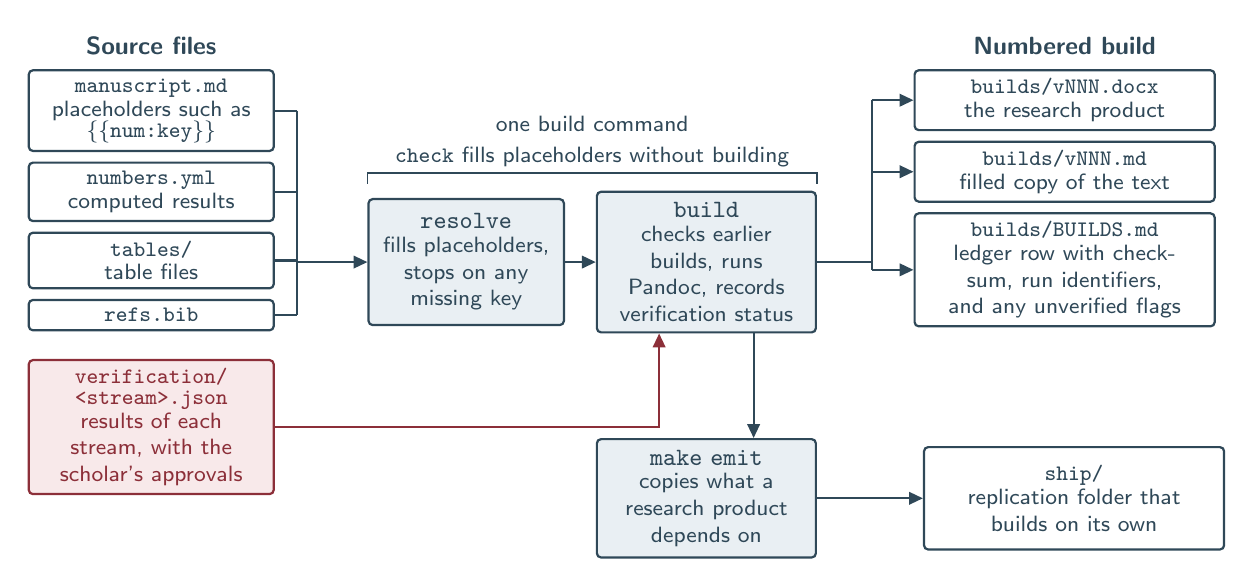
\begin{tikzpicture}
\tikzset{
  file/.style={box, draw=cslate, fill=white, text=cslate, inner sep=3pt, font=\fontsize{8}{9.6}\selectfont},
  mod/.style={pipe, minimum height=1.6cm, font=\fontsize{8}{9.6}\selectfont},
}
\newcommand{\nm}[1]{{\fontsize{9}{11}\selectfont\ttfamily #1}}
\newcommand{\fn}[1]{{\fontsize{8}{9.4}\selectfont\ttfamily #1}}
\newcommand{\sm}[1]{{\fontsize{8}{9.4}\selectfont #1}}
% inputs
\node[font=\fontsize{9}{11}\selectfont\bfseries, text=cslate] at (1.7,2.75) {Source files};
\node[file, text width=2.9cm, anchor=north] (in1) at (1.7,2.45) {\fn{manuscript.md}\\[-1pt]\sm{placeholders such as}\\[-2pt]\fn{\{\{num:key\}\}}};
\node[file, text width=2.9cm, anchor=north] (in2) at ($(in1.south)+(0,-0.12)$) {\fn{numbers.yml}\\[-1pt]\sm{computed results}};
\node[file, text width=2.9cm, anchor=north] (in3) at ($(in2.south)+(0,-0.12)$) {\fn{tables/}\\[-1pt]\sm{table files}};
\node[file, text width=2.9cm, anchor=north] (in4) at ($(in3.south)+(0,-0.12)$) {\fn{refs.bib}};
\node[ver, text width=2.9cm, anchor=north, font=\fontsize{8}{9.6}\selectfont, inner sep=3pt] (in5) at ($(in4.south)+(0,-0.35)$) {\fn{verification/}\\[-2pt]\fn{<stream>.json}\\[-1pt]\sm{results of each stream, with the scholar's approvals}};
% modules
\node[mod, text width=2.2cm] (res) at (5.7,0) {\nm{resolve}\\[-1pt]\sm{fills placeholders, stops on any missing key}};
\node[mod, text width=2.5cm] (bld) at (8.75,0) {\nm{build}\\[-1pt]\sm{checks earlier builds, runs Pandoc, records verification status}};
\draw[cslate, line width=0.6pt] (res.north west)++(0,0.18) -- ++(0,0.14) coordinate (bl) -- (bl -| bld.north east) -- ++(0,-0.14);
\node[anchor=south, inner sep=1pt, align=center, text=cslate] at ($(bl)!0.5!(bl -| bld.north east)+(0,0.04)$) {\sm{one build command}\\[-1pt]\sm{\texttt{check} fills placeholders without building}};
% outputs
\node[font=\fontsize{9}{11}\selectfont\bfseries, text=cslate] at (13.3,2.75) {Numbered build};
\node[file, text width=3.6cm, anchor=north] (out1) at (13.3,2.45) {\fn{builds/vNNN.docx}\\[-1pt]\sm{the research product}};
\node[file, text width=3.6cm, anchor=north] (out2) at ($(out1.south)+(0,-0.12)$) {\fn{builds/vNNN.md}\\[-1pt]\sm{filled copy of the text}};
\node[file, text width=3.6cm, anchor=north] (out3) at ($(out2.south)+(0,-0.12)$) {\fn{builds/BUILDS.md}\\[-1pt]\sm{ledger row with checksum, run identifiers, and any unverified flags}};
% replication folder
\node[mod, text width=2.5cm, minimum height=1.3cm] (emit) at (8.75,-3.0) {\nm{make emit}\\[-1pt]\sm{copies what a research product depends on}};
\node[file, text width=3.6cm, anchor=west, minimum height=1.3cm] (ship) at (11.5,-3.0) {\fn{ship/}\\[-1pt]\sm{replication folder that builds on its own}};
% wiring
\coordinate (ib) at (3.55,0);
\foreach \n in {in1,in2,in3,in4} {\draw[line width=0.8pt, cslate] (\n.east) -- (\n.east -| ib);}
\draw[line width=0.8pt, cslate] (in1.east -| ib) -- (in4.east -| ib);
\draw[flow, cred] (in5.east) -- ($(in5.east -| bld.south)+(-0.6,0)$) -- ($(bld.south)+(-0.6,0)$);
\draw[flow, cslate] (ib) -- (res.west);
\draw[flow, cslate] (res.east) -- (bld.west);
\coordinate (ob) at (10.85,0);
\draw[line width=0.8pt, cslate] (bld.east) -- (ob);
\draw[line width=0.8pt, cslate] (out1.west -| ob) -- (out3.west -| ob);
\foreach \n in {out1,out2,out3} {\draw[flow, cslate] (\n.west -| ob) -- (\n.west);}
\draw[flow, cslate] ($(bld.south)+(0.6,0)$) -- ($(emit.north)+(0.6,0)$);
\draw[flow, cslate] (emit.east) -- (ship.west);
\end{tikzpicture}
\end{document}
